
\documentclass[final,  3p]{elsarticle}

\usepackage{csvsimple}
\usepackage{amssymb, amsthm}
\usepackage{amsmath}
\usepackage{subcaption}
\usepackage[T1]{fontenc}
\usepackage{babel}
\usepackage{wrapfig}
\usepackage{geometry}
\usepackage{fancyref}
\usepackage{lineno}
\usepackage{color}
\usepackage{nomencl}
\usepackage{tabularx}
\makenomenclature
\renewcommand{\nomlabel}[1]{\hfil #1\hfil}

\journal{}

\begin{document}

\begin{frontmatter}

\title{Investigation of Limited Detection Schemes for Light Scattering of Optically Trapped Asymmetric Particles}


\author[aff1]{Daniel Maciver\corref{cor1}} 
\ead{Daniel.Maciver.2016@uni.strath.ac.uk}

\author[aff1]{Praveen Parthasarathi}

\author[aff1]{Leo Lue}

\author[aff1]{Jan Sefcik}

\author[aff1]{Mark Haw}

\cortext[cor1]{Corresponding author}
\affiliation[aff1]{organization={Department of Chemical Engineering,
			University of Strathclyde},
            addressline={75 Montrose Street}, 
            city={Glasgow},
            postcode={G1 1XL}, 
            country={Scotland}}
        
\begin{flushright}
	Daniel Maciver \\
	daniel.maciver.2016@uni.strath.ac.uk \\
	University of Strathclyde, \\
	75 Montrose Street, \\
	Glasgow, \\
	G1 1XL \\
	07793445441 
\end{flushright}

\begin{abstract}
  % \justifying
  %
  While optical trapping is a well understood method for force
  transduction and detection, further characterisation of trapped entities using light-scattering
  poses a two-fold challenge --- one experimental, concerning the optimal
  arrangement of light detectors to gather data and minimising signal noise, and the other theoretical, involving
  solving of the inverse light scattering problem in order to interpret this data. Experimentally, combining static
  light scattering techniques with optical trapping poses significant
  engineering challenges due to the space constraints in a
  conventional optical trapping setup.  We propose here a plausible
  scenario of detecting scattered light from an optically trapped
  asymmetric microstructure using a novel, multi-angle, optical-fibre
  based detection scheme and demonstrate how a Bayesian inference
  based analysis of the data, combined with a neural-network trained on data simulated to mimic light scattering
  detection signals in such scenarios, may be used for solving the
  inverse light scattering problem and characterising complex trapped
  entities.  To demonstrate the method we discuss its application to
  measuring the instantaneous orientations of a trapped asymmetric microsphere
  dimer. We argue that the method can be extended to
  determine any characteristics of the trapped microstructure that
  influence the light scattering pattern.
\end{abstract}
	
%\begin{highlights}
%\item Asymmetric microsphere dimers can undergo complex dynamics including full inversions in the presence of a trapping potential, depending sensitively on the size ratio of the spheres making up the dimer.  
%\item Orientations can be inferred from scattering signals through classification by a combination of neural networks and Bayesian inference. 
%\item Signal error has a significant effect on the performance of the neural network, which can be countered via biasing of the prior distribution. 
%\item Future applications include continuous processes where trapped particle characteristics such as size and shape are changing with time.  
%\end{highlights}

\begin{keyword}
	Optical Trapping \sep Light Scattering \sep Measurements \sep Bayesian Statistics 
\end{keyword}

\end{frontmatter}
\newpage
%%%%%%%%%%%%%%%%%%%%%%%%%%%%%%%%%%%%%%%%%%%%%%%%%%%%%%%%%%%%%%%%%%%%%
%%%%%%%%%%%%%%%%%%%%%%%%%%%%%%%%%%%%%%%%%%%%%%%%%%%%%%%%%%%%%%%%%%%%%
%%%%%%%%%%%%%%%%%%%%%%%%%%%%%%%%%%%%%%%%%%%%%%%%%%%%%%%%%%%%%%%%%%%%%

\section{Introduction}
\label{sec:Intro}

Since their invention in the late 1980s, optical tweezers have found application in experiments ranging from single molecule biophysics \cite{Bustamante2021Biophysics} to testing the fundamental assumptions of quantum mechanics \cite{yin2013large}, thanks mainly to the ability of the tweezer to transduce and detect forces on the order of a few pico-newtons. Going beyond forces, further structural, dynamic and chemical characterisation of complex trapped entities could provide useful information, as demonstrated in areas such as metrology \cite{arita2020coherent} and colloidal aggregation \cite{burns1990optical}.  Spectroscopic techniques such as Raman scattering \cite{gupta2014raman} have been used for chemical characterisation of trapped objects, while dynamical characterisation has been demonstrated using data from tweezer's Quadrant Photo Detector (QPD) by following the centre-of-mass Brownian motion of the trapped entity \cite{friedrich2012tuning} and measuring rotation of the centre-of-mass\cite{yifat2021facile}.  A recent work aimed at characterising trapped entities demonstrated how neural networks maybe trained to distinguish between optically trapped micro-beads of different size and material by means of a principal component analysis of the forward scattered light detected using a QPD \cite{Carvalho_2023}. A more direct, albeit cumbersome attempt at detecting scattered light from trapped biological cells was attempted in \cite{Watson_2023} where the experimental cuvette was placed inside an elliptical mirror that directed light scattered from the trapped biological-cell onto a photodetector via a rotating aperture that helped select the scattering-angle. Thus, past studies on optical trapping have focused on either on particle trapping to study trapping dynamics, or on the characterisation of particles with relatively simple complex trapping dynamics.  

While both \cite{Carvalho_2023} \cite{Watson_2023} demonstrate some ability to characterise trapped entities, \cite{Carvalho_2023} is perhaps best suited to characterise micron-sized particles with simple trapping dynamics, and \cite{Watson_2023} talks about an experimental setup that is difficult to adopt and suffers from a low-bandwidth that might not be best suited for monitoring dynamics. A light scattering detection scheme built around an optical trap that is both easy to implement and has the advantage of high-bandwidth was demonstrated by Safran and co-workers in \cite{Bar-Ziv_1998}, where a single-mode optical fibre was aligned to detect the scattered light from a trapped bead and study its Brownian motion - commonly now refereed to as Localised dynamic light scattering (LDLS). This was later expanded upon by \cite{PhysRevE.65.041921} by collecting back scattered light to characterise the Stokes friction coefficient as a function of trapping depth. While both papers provided dynamical information, structural information about the trapped bead was precluded as the scattered wave was only measured across a small angular range. Furthermore, the main drawback to a LDLS is that it struggles to characterise asymmetric particles such as nano rods or dimers; in which case the Brownian motion is no longer simply translational, but rotational about the centre of mass \cite{yin2013large}.

One way of mitigating this is to remove translational fluctuations from the analysis; by monitoring its the scattering, Cang and co-workers were able to spatially fix a gold nanorod at the centre of trapping laser by moving the sample plane accordingly, to an accuracy of 200 nm \cite{Cang2006}. However, this has limited application's to anisotropic scatters such as biological matter where the internal structure of many cells makes them inherently anisotropic \cite{Watson_2023}. Thus even if the Cartesian coordinates are relatively fixed characterisation of the scattering pattern will have to separate the contributions of internal structure and orientation. In this work, we propose a scheme that expands on the technique in \cite{Bar-Ziv_1998} to detect scattered light simultaneously at a number of angles (Figure 1), combined with a novel Bayesian inference-based analysis technique, to enable interpretation of the resulting multi-angle data from an anisotropic, asymmetric scatterer, as well as optimisation to provide maximal information from the signal. 

To demonstrate the analysis, we study a simple, illustrative example of an anisotropic scattering entity \emph{i.e.} an asymmetric dimer. As a paradigmatic example of extracting structural/dynamic information from the resulting scattering data, we explore how to estimate the dimer's instantaneous orientation from the scattering signals using Bayesian inference, as well as how to optimise the analysis by implementing 'prior knowledge' to obtain the most reliable estimate. As an example of the relatively sparse literature on measuring orientations of complex trapped objects, \cite{raudsepp2022estimating} employs imaging to study the orientation of trapped dimers: scattering can give more quantitative and potentially more rapid time-resolved information, but only of course if the scattering signals can be interpreted. Here, we first train a neural network to effectively identify the mapping between scattering signals and dimer orientation, by calculating the scattering signal from a simulated asymmetric dimer undergoing Brownian motion in an optical trap and mapping to the known instantaneous orientation of the simulated dimer. We then show how Bayesian inference can be used to optimise extraction of the true dimer orientation from the light scattering signals. Furthermore we demonstrate how the model's performance when dealing with signal noise, a common problem when analysing scattering behaviour. 

\begin{figure} [b]
\centering
\begin{subfigure}{0.45\textwidth}
	\subcaption{}
	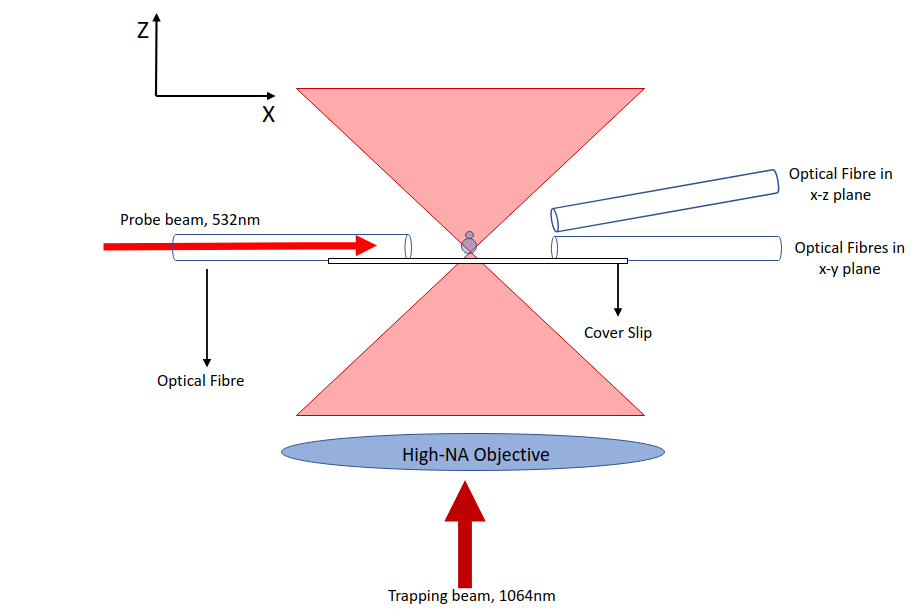
\includegraphics[width=\textwidth, height=0.25\textheight]{./Images/fig1a.png}
\end{subfigure}
\begin{subfigure}{0.45\textwidth}
	\subcaption{}
	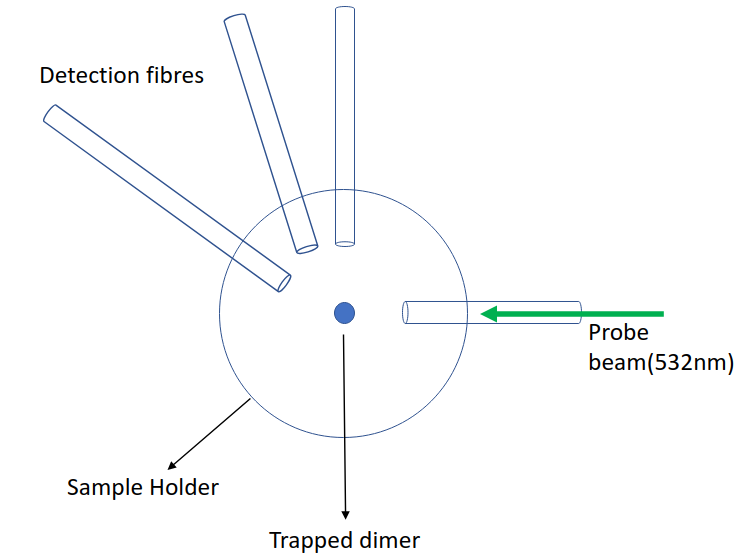
\includegraphics[width=\textwidth, height=0.25\textheight]{./Images/fig1b.png}
\end{subfigure}
\caption{\label{fig:setup}
  %
  Proposed experimental set up for scattering measurements from an object in an optical trap. The probe beam for scattering measurements is incident perpendicular to the trapping laser propagation direction. a) Side view. b) Top view. Note that three of the detector fibres are co-planar with the incident probe beam, while the fourth detector is placed out of the plane (see Sec~\ref{sec:detectors}).
%
}
\end{figure}

%%%%%%%%%%%%%%%%%%%%%%%%%%%%%%%%%%%%%%%%%%%%%%%%%%%%%%%%%%%%%%%%%%%%%
%%%%%%%%%%%%%%%%%%%%%%%%%%%%%%%%%%%%%%%%%%%%%%%%%%%%%%%%%%%%%%%%%%%%%
\section{Methodology}
\label{sec:Method}
\subsection{Orientation estimation from scattering measurements}
\label{sec:Bayes}

Consider a dimer in the optical trap (Fig.~\ref{fig:dimer}a), we can define at any point in time a unit vector $\hat{s}$ pointing from the centre of the larger sphere to the centre of the smaller sphere. A plane wave 'probe' laser, perpendicular to the trapping laser, is incident on the dimer, generating a scattering pattern  dependent on the dimer's orientation $I(\hat{\bf s}, \theta)$ which can be computed using  software such as MSTM \cite{Mishchenko1996MSTM}. To represent the experimental set up consisting of a set of optical fibres recording scattered light, we choose four angles  ($\theta_1, \ \theta_2, \ \theta_3, \ \theta_4$) and record the calculated intensity at each angle $\theta_k$, $I(\hat{s}, \theta_k)$. 

\begin{figure}[h]
	\centering
	\begin{subfigure}{0.49\textwidth}
		\subcaption{}
		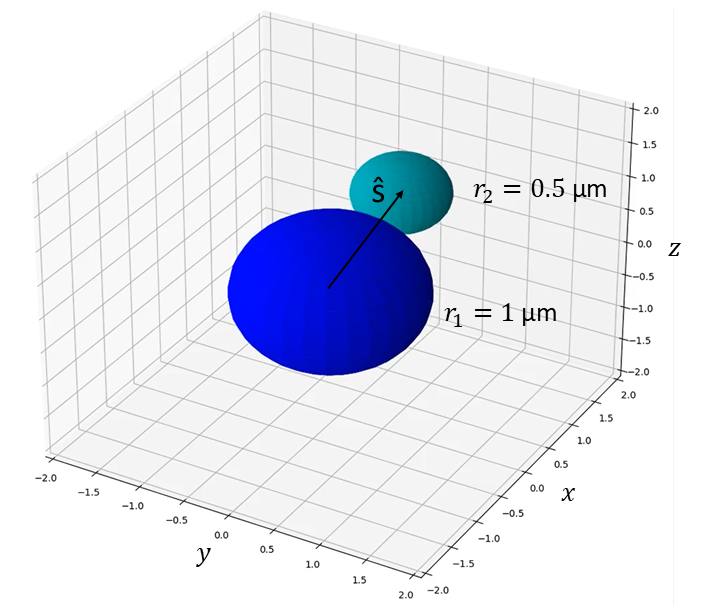
\includegraphics[width=\textwidth]{./Images/fig2a.png}
	\end{subfigure}
	\begin{subfigure}{0.49\textwidth}
		\subcaption{}
		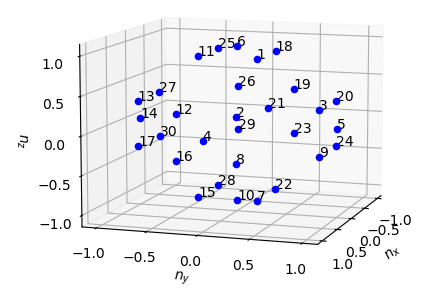
\includegraphics[width=\textwidth]{./Images/fig2b.png}
	\end{subfigure}
	\caption{(a)Example dimer in orientation $\bar{\bf s}$, (b) 30 Reference orientations represented by vectors pointing from [0,0,0] to each point}
	\label{fig:dimer}
\end{figure}

Our goal is to determine the orientation of the trapped dimer based on the measured intensity $I(\hat{n}, \ \theta_k)$. Rather than aim immediately for an exact estimate of the dimer's orientation, for the purposes of interpretation of the scattering and optimisation of the measurement setup it is more convenient to discretize the possible orientation space into a number of possible reference orientations, which we can then use as 'classification categories' in a neural network methodology to map scattering data to orientation (see below for further discussion).  Here we choose $\textit{n}_{ref} \ = \ 30$ reference orientations $\hat{\bf n}_{\alpha}$  evenly distributed on a unit sphere \cite{Rey2006} (Figure~\ref{fig:dimer}b) leading to a maximum nearest-neighbour spacing between two neighbouring reference orientations of 0.895 radians. Using MSTM we compute the raw intensities at each of the measurement angles that would be generated by a dimer in each reference orientation, $I(\hat{\bf n}_{\alpha}, \theta_k)$. While the number and position of detection fibres is technically arbitrary there are several constraining factors that limit our ability to infer useful information from the trapped object, see Section~\ref{sec:detectors} for a detailed breakdown of our choice of detection angles. The raw intensities are normalized according to:
\begin{align}
\label{eq:scale}
  y_k(\hat{\bf n}_\alpha)
  = 
  \frac{I(\hat{\bf n}_\alpha, \theta_k) - \langle I(\hat{\bf n},\theta_k) \rangle } 
  {\langle I^2(\hat{\bf n},\theta_k) \rangle -\langle I(\hat{\bf n}, \theta_k)\rangle^2}
\end{align}
where the denominator is simply the standard deviation across the set of values $I(\hat{\bf n}, \theta_k)$. The reference orientations, raw intensities, and scaled signals are given in Tables~\ref{tab:A1} and \ref{tab:A2}. 

Note that the collected scattering signals are not necessarily simply related to their associated reference orientations: as is well known from such examples of the inverse scattering problem. While it is trivial to compute the light scattering pattern for any given particle with any particular characteristic (i.e. size, shape, or orientation), inferring the light scattering from a unknown particle to determine said characteristic is incredibly difficult due to complex mapping between scattering and said characteristic. Even if the orientation space is divided evenly between reference orientation the subsequent signal space ends up being appearing mixed making simple comparisons of signals useless for inferring information on the particle. Shown below is two clusters of orientation vectors and there respective measured scattering signals - the points have been coloured based on their proximity to the centre of their respective cluster. While the orientation space appears tightly packed and ordered the signal space quickly spreads out in an asymmetric fashion. Furthermore as seen in Fig~\ref{fig:mixing}b the signal mapping can intersect itself which only further increases the complexity. While in some instances the mapping between one reference orientation and another is discrete, in other instances the mapping becomes far more complex to discern. 

\begin{figure}[h]
	\centering
	\begin{subfigure}{0.4\textwidth}
		\subcaption{}
		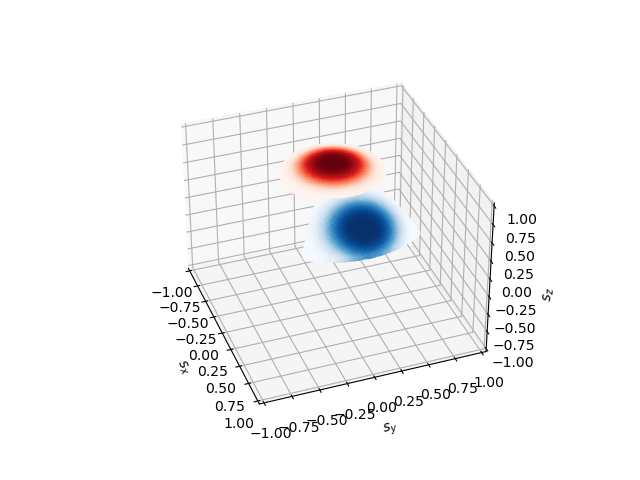
\includegraphics[width=\textwidth]{./Images/fig3a.png}
	\end{subfigure}
	\begin{subfigure}{0.4\textwidth}
		\subcaption{}
		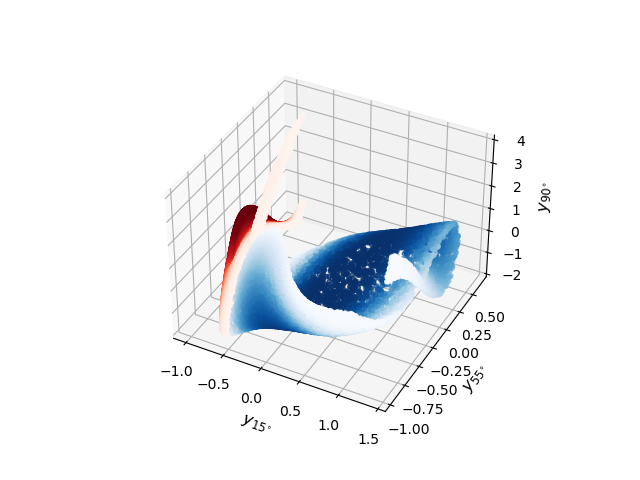
\includegraphics[width=\textwidth]{./Images/fig3b.png}
	\end{subfigure}
	\caption{(a) Distribution of orientation vectors and (b) their respective scattering signals. Points are coloured according to their distance from the centre of each cluster (red points centred around [$0.00, 0.00, 1.00$], blue points centred at [$0.71, 0.00, 0.71$])}
	\label{fig:mixing}
\end{figure}

Nevertheless, at least where the uncertainty in signal measurements is low (see below), we can predict the orientation from the scattering by utilising computational techniques such as neural networks. We thus utilised the Python machine learning program \textit{scikit-learn} to build a neural network for identifying the dimer's orientation from its light scattering signal. The network was trained by generating a database of random orientation vectors, calculating the corresponding light scattering signals, and then using the network to estimate the probability of a given signal coming from a dimer in a given reference orientation. The network's loss function was evaluated and used to improve the estimation, the network being trained until the improvement in the loss function was less than 0.0001. 
%
Importantly, the estimation provided by the neural network can be improved further by accounting for any prior information we know about the dimer, utilising Bayesian inference to update the neural network's estimation: 

\begin{align}
  \label{eq:bayes}
  p(\hat{\bf n}_\alpha| y_k(\hat{\bf s}))
  &=
    \frac{p(y_k(\hat{\bf s})|\hat{\bf n}_\alpha)
    p(\hat{\bf n}_\alpha)}{p(y_k(\hat{\bf s}))}
\end{align}
where $p(\hat{\bf n}_\alpha)$ and $p(y_1, y_2, y_3)$ are the prior estimates of the distributions of particle orientations and instantaneous signals, respectively.
\textit{Without} any prior evidence we must assume that the orientation prior of the dimer
$p(\hat{\bf n}_{\alpha})$ is uniform. However, inference about the dimer's possible current orientation from knowledge of previous
measurements can be used to inform our estimate of $p(\hat{\bf n}_{\alpha})$ (see Section~\ref{sec:test}). The latter prior $p(y)$ is the probability of measuring a signal ($y_1$, $y_2$, $y_3$).  This is given by taking the discrete integral over the collection of reference orientations:
\begin{align}
  p(y_1, y_2, y_3, y_4)
  =
  \sum_{\alpha=1}^{n_{\rm ref}}
  p(y_1, y_2, y_3, y_4|\hat{\bf n}_\alpha)
  p(\hat{\bf n}_\alpha)
\end{align}
From \eqref{eq:bayes} we obtain the key result, a mass probability distribution denoting the
probability that our dimer is in orientation $\hat{\bf n}_{\alpha}$ given a measured
signal ($y_1$, $y_2$, $y_3$), \textit{i.e.} an estimated mapping from scattering measurement to orientation estimate. 

%%%%%%%%%%%%%%%%%%%%%%%%%%%%%%%%%%%%%%%%%%%%%%%%%%%%%%%%%%%%%%%%%%%%%
\subsection{Calculation of error}
\label{sec:divergence}
To evaluate the above estimation of dimer orientation from scattering signal, we use a Brownian simulation of a dimer in the optical trap (Section~\ref{sec:brownian}) to compare estimated most probable reference orientation, derived from the dimer's scattering through Eq.~\eqref{eq:bayes}, with the dimer's known \emph{actual} orientation $\hat{\bf s}$. MSTM provides calculated light scattering from the simulated dimer $I(\hat{\bf s}, \theta)$ and we use \eqref{eq:scale} to obtain normalized values at each measurement angle $\theta_k$,  $y_1(\hat{\bf s})$, $y_2(\hat{\bf s})$, $y_3(\hat{\bf s})$, from which we obtain $p(\hat{\bf n}_{\alpha}\parallel y_1, y_2, y_3)$. Because we know the actual orientation $\hat{s}$ we can measure the error in the model's estimate by comparing the reference orientation closest to $\hat{s}$, denoted as $\hat{\bf n}_{best}$, with the most probable predicted orientation from Eq.~\eqref{eq:bayes}. An ideal result would be one where the probability distribution is 0 for every $\hat{\bf n}$ apart from $\hat{\bf n}_{best}$:
\begin{align}
	\label{eq:best}
	p_{best} = 
	\begin{cases}
		1 & \text{when $\hat{\bf n}_\alpha$ = $\hat{\bf n}_{best}$}\\
		0 & \text{anywhere else}
	\end{cases}
\end{align}
In reality the distribution from Eq.~\eqref{eq:bayes} will assign some non-zero
probability to every reference orientation, leading to some level 'confidence' in orientation prediction, which can be quantified by calculating the Kullback-Leibler divergence $K_l$ between the two distributions:
\begin{align}
	K_{l, \#}(p_{best}\parallel p(\hat{\bf n}_\alpha| y_1, y_2, y_3))
	= p_{best}\ln \left[\frac{p_{best}}{p(\hat{\bf n}_{best}| y_1,y_2,y_3))}
	\right]
	\label{eq;kullback}
\end{align}
where a larger value of $K_l$ indicates that our model is less confident in its
prediction of the dimer's orientation. The divergence $K_l$ thus illustrates the 'spread'
in the estimated dimer orientation probability --- a distribution strongly peaked at 
some value would give us more confidence in that value than a near-uniform distribution 
where the scattering measurement could imply a wide range of possible orientations --- 
but it does not directly indicate our estimates actual accuracy, that can be simply defined as the percentage of our estimations that are correct. 

%%%%%%%%%%%%%%%%%%%%%%%%%%%%%%%%%%%%%%%%%%%%%%%%%%%%%%%%%%%%%%%%%%%%%
%%%%%%%%%%%%%%%%%%%%%%%%%%%%%%%%%%%%%%%%%%%%%%%%%%%%%%%%%%%%%%%%%%%%%
\subsection{Brownian Simulation}
\label{sec:brownian}

We use the Brownian OT package developed by Fung~\textit{et~al} \cite{Vigilante2020Brownian_OT} to simulate the motion of an asymmetric dimer (Figure~\ref{fig:dimer}a) within an optical trap. Brownian OT combines MSTM \cite{Mishchenko1996MSTM} and ``Optical Tweezer Toolbox'' (\textit{ott}) \cite{Lenton2020} to simulate the motion of arbitrary
shaped sphere clusters. We simulate the motion of a dimer trapped in a highly focused Gaussian beam by calculating the optical forces imparted by the laser, and the Brownian force due to the surrounding fluid. MSTM provides the necessary T-matrix to compute the optical force via \textit{ott}. The Brownian force is found by computing the dimer's diffusion tensor according to the analytical solutions provided by Nir and Acrivos \cite{nir_acrivos_1973}. We simulated a polystyrene dimer ($n = 1.59$) in a suspension of water ($n_{med} = 1.33$) over the course of $1 \ s$ with a simulation time step of $1 \times 10^{-5} \ s$. We placed the dimer 4 microns below the trap focus at an angle $30^{\circ}$ from the horizontal, the resulting trajectory is shown below in Sec~\ref{sec:motion}. We chose these initial parameters because it demonstrates our model's performance in non steady state conditions. 

%%%%%%%%%%%%%%%%%%%%%%%%%%%%%%%%%%%%%%%%%%%%%%%%%%%%%%%%%%%%%%%%%%%%%
%%%%%%%%%%%%%%%%%%%%%%%%%%%%%%%%%%%%%%%%%%%%%%%%%%%%%%%%%%%%%%%%%%%%%
\section{Results and  Discussion}
\label{sec:Discussion}
\subsection{Minimal number of detectors}
\label{sec:detectors}
The exact number of detectors was initially assumed to be arbitrary, in that it made no difference to our estimate whether we used 2 angles or 200. For practical purposes it seemed beneficial that we demonstrate our method works for a minimal number of detection angles, as geometric constraints come into play when trying to install a high number of detection fibres for any optical tweezer set up. 

\begin{figure}[h]
	\centering
	\begin{subfigure}{0.49\textwidth}
		\subcaption{}
		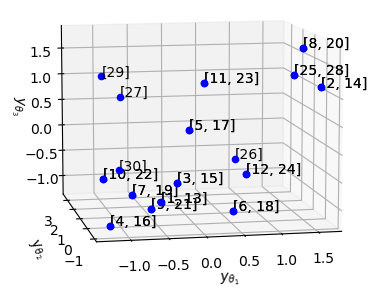
\includegraphics[width=\textwidth]{./Images/fig4a.png}
	\end{subfigure}
	\begin{subfigure}{0.4\textwidth}
		\subcaption{}
		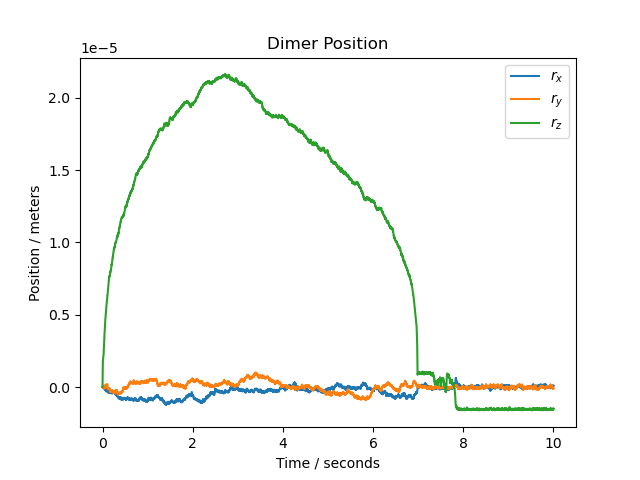
\includegraphics[width=\textwidth]{./Images/fig4b.png}
	\end{subfigure}
	\caption{Expected scattered signals from reference orientations -see fig~\ref{fig:dimer} - when: (a) all three detectors are in the X-Y plane, (b) when 1 detector is raised out of the X-Y plane.}
	\label{fig:detectors}
\end{figure}

 When all of the detectors lie in the same plane the expected signal can appear identical despite the dimer being in completely different orientations. This is shown in Figure~\ref{fig:detectors} which plots the expected signals from 30 reference orientations, each point is labelled with its corresponding reference orientation, the fact that points have multiple labels is because the dimer's scattering is indistinguishable in these two reference orientation. It should be noted that these pairs are reflected in one or more axis which suggests that these are due to the arrangement of our detectors. More specifically, if the detectors are placed say in the x-y plane then only when the dimer is pointed nearly fully upright will the expected signal be entirely unique. This is illustrative of the difficulty behind the inverse light scattering problem; as one cannot always map a given signal to a particular parameter value.

To remedy this we raise the third detector out of the x-y plane; as such the expected signals from each reference orientation is unique. As seen between Figures \ref{fig:detectors}a \& b each reference orientation now has a unique scattering signal, though with only three detectors the difference in expected signals can appear insignificant. By adding a $4^{th}$ detector we can differentiate signals more reliably, improving the neural networks performance.   In line with our goal of making this method viable in a laboratory setting we decided not to increase the number of detectors further than 4. 

%%%%%%%%%%%%%%%%%%%%%%%%%%%%%%%%%%%%%%%%%%%%%%%%%%%%%%%%%%%%%%%%%%%%%
\subsection{Testing the Model}
\label{sec:test}
Using our simulation from Section~\ref{sec:brownian} we simulated the motion of a silica dimer ($n = 1.45$) trapped in water ($n = 1.33$) within a 5 mW optical trap. The trapping laser is 1064nm NIR focused through a 1.25 NA objective. The dimer is comprised of two tangent spheres with radii $1 \mu m$ and $0.5 \mu m$ respectively. We simulated the first 10 seconds of motion, calculating the orientation and position every 1 ms. 

We applied Eq.~\eqref{eq:bayes}, taking the reference orientation with the highest probability  as our estimate of the dimer's instantaneous orientation $\hat{\bf n}_{est}$. To visualise the model's performance  we plotted the radial distance between our estimation $\hat{\bf n}_{est}$ and the dimer's \emph{actual} instantaneous orientation $\hat{\bf s}$ versus time. For comparison, we also plotted the radian distance between the  dimer's instantaneous orientation and the closest reference orientation, denoted $\hat{\bf n}_{best}$. The dotted line indicates the maximum radian distance ($0.896$ radians) between two \textit{neighbouring} reference orientations: if we are under this line then we know our estimate is at least neighbouring the best result. Assuming a uniform prior of the reference orientations $p(\hat{\bf n}_\alpha)$  the neural network's predictions ($\hat{\bf n}_{est}$ from Eq.~\eqref{eq:bayes}) are at times reasonable, but there are significant large and random jumps away from the correct result (Fig.~\ref{fig:uniform}). 

\begin{figure}[h]
	\centering
	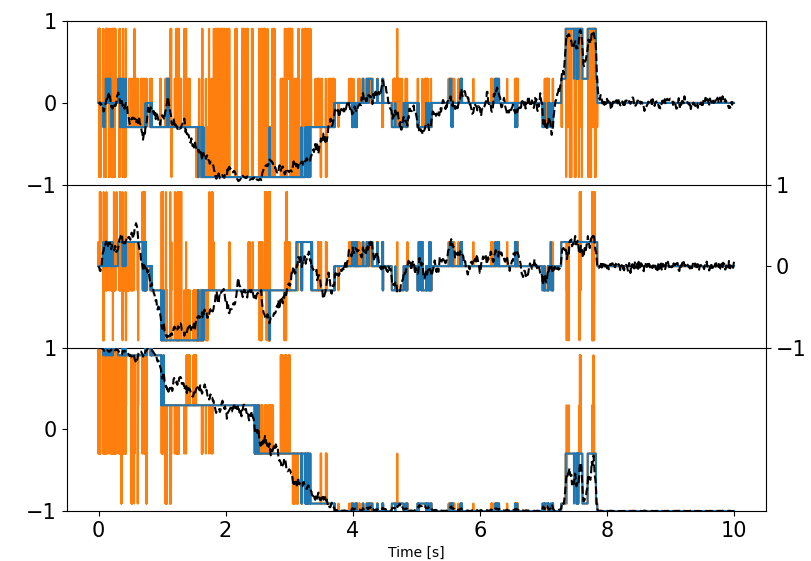
\includegraphics[width=0.5\textwidth]{./Images/fig5.png}
	\caption{Model's estimation of dimer orientation over the simulation time, assuming uniform prior $p(\hat{\bf n}_\alpha)$, broken up into x, y, and z components for clarity. Blue line denotes the best result we can achieve (the reference orientation $\hat{\bf n}_{best}$ that is closest to the actual orientation), orange line denotes the result provided by eq~\ref{eq:bayes}: where the orange line is not visible, the model's prediction agrees with $\hat{\bf n}_{best}$. Dotted black line is the instantaneous orientation $\hat{\bf s}$.}
	\label{fig:uniform}
\end{figure} 

One reason we observe such large jumps in orientation estimated from scattering signals is that there is no simple correlation between the 'distance in scattering space' between scattering signals from two different orientations, and their separation in orientation space: even a large change in orientation can involve a small change in scattering. Combining this fact with use of a uniform prior, indicating essentially no knowledge of how orientation should behave, there is no constraint on how much estimated orientation can change from time-step to time-step. To improve the estimation we can therefore use knowledge of the physical limitations of the object in the trap and its dynamics, imposing a more physically grounded prior, accounting in this case for the fact that the motion of the dimer is limited due to the trap stiffness. Here the prior of the reference orientations $p(\hat{\bf n}_\alpha)$ was redefined at each time step as a Boltzmann distribution of the physical distance between the previous estimate $\hat{\bf n}_{est}(t-\Delta t)$ and each reference orientation $\hat{\bf n}_\alpha$. Put simply, we are reweighing our estimation based on the size of rotation required, with smaller movements being favoured over large movements:

\begin{align}
  p(\hat{\bf n}_\alpha)
  &=\frac{e^{\beta (\hat{\bf n}_\alpha 
  	\cdot \hat{\bf n}_{est}(t-\Delta t))}}
  {\sum_{\alpha=1}^{n_{\rm ref}}
	e^{\beta (\hat{\bf n}_\alpha 
	\cdot \hat{\bf n}_{est}(t-\Delta t)}}
	\label{eq:boltz}
\end{align}
Here $\beta$ is a weighting factor describing the dimer's freedom of motion within the trap. As shown in Figure~\ref{fig:biased} implementation of Eq~\eqref{eq:boltz} helps significantly reduce the large random excursions of estimated orientation away from the 'best' result. 

\begin{figure}[h]
\centering
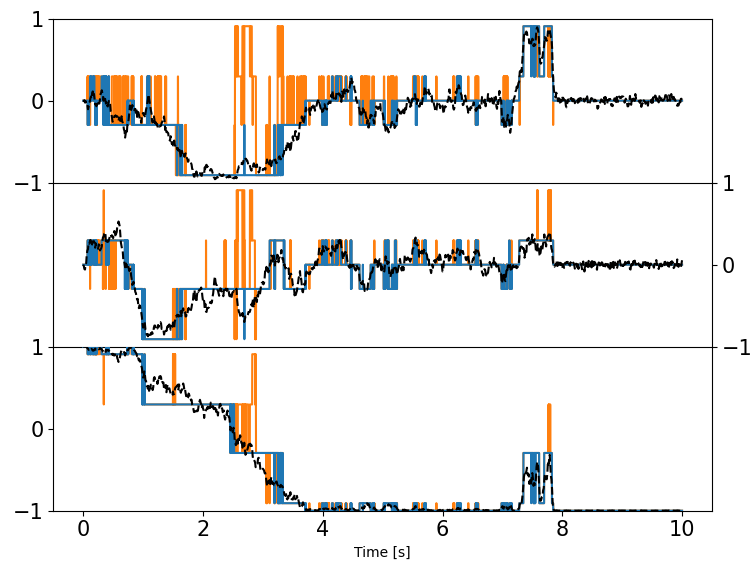
\includegraphics[width=0.5\textwidth]{./Images/fig8a.png}
\caption{\label{fig:biased}
%
Estimation of dimer orientation with $p(\hat{\bf n}_\alpha)$ defined
by Eq~\eqref{eq:boltz}.  Blue line denotes the best result we can
achieve, orange line denotes the result provided by eq~\ref{eq:bayes}.
Dotted black line is the instantaneous orientation $\hat{\bf s}$ (see Section~\ref{sec:Bayes}).
  %
}
\end{figure} 

The simulation data from Section~\ref{sec:brownian} was used to evaluate our model's performance --- covered in Section~\ref{sec:divergence}. By summing the divergence of each measurement across the entire simulation we get an evaluation of how well the model performed in estimating the dimer's orientation. To compare the effects of changing certain parameters on the performance of our model we compare our result of $K_{l,total}$ to a worst case scenario and evaluate how much it improves upon this, denoted as $F(K_l)$:
\begin{align}
  K_{l, \ total} &= \sum\limits_{\# =1}^{timesteps} K_{l,\#}
  \\
  K_{l, \ worst} &= \sum\limits_{\#=1}^{timesteps} \ln \left[\frac{1}{1/n_{ref}} \right]
  \\
  F(K_l) &= \frac{K_{l,\ worst}}{K_{l, \ total}}
\end{align}

The worst case scenario is akin to randomly choosing a reference
orientation at each time step. The greater the value of $F(K_l)$, the
better our model's confidence is in characterising the dimer's
motion. Because our model is dependent on several parameters we need
to a sophisticated method for understanding how these parameters
correlate with $F(K_l)$.

%%%%%%%%%%%%%%%%%%%%%%%%%%%%%%%%%%%%%%%%%%%%%%%%%%%%%%%%%%%%%%%%%%%%%
\subsection{Asymmetric dimer dynamics}
\label{sec:motion}

The Brownian OT software was used to simulate the motion of a trapped dimer ($a_1=1\,\mu{\rm m}$, $a_2=0.5\,\mu{\rm m}$) over the first $1$ seconds of entering the optical trap.  The initial orientation was set at $s = (0.923, 0.0, 0.385)$. The dimer's position and orientation was recorded every $10\,{\rm \mu s}$ for using as a test dataset for our model.

\begin{figure}[h]
	\centering
	\begin{subfigure}{0.45\textwidth}
		\subcaption{}
		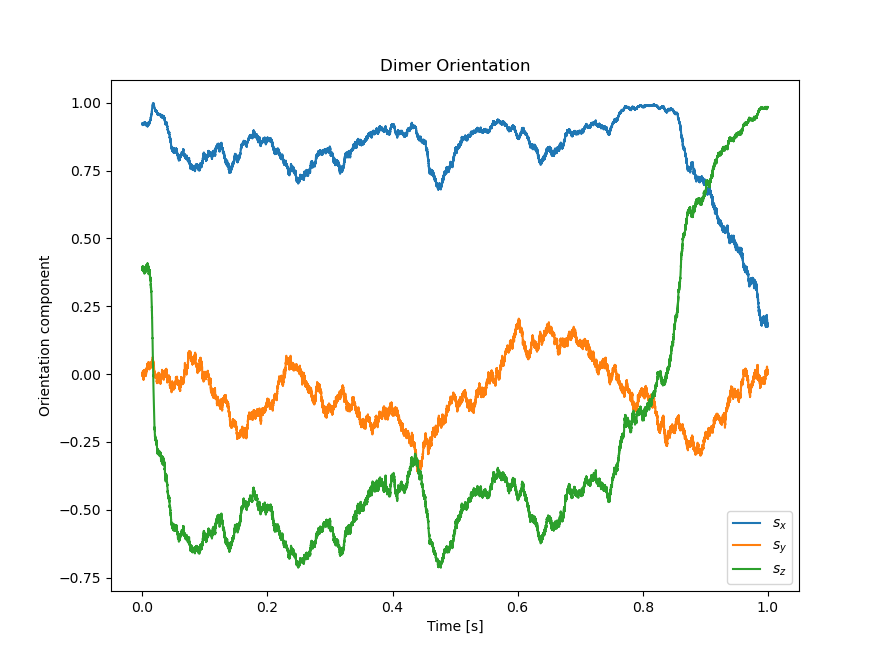
\includegraphics[width =\textwidth]{./Images/fig7a.png}
	\end{subfigure}
	\begin{subfigure}{0.45\textwidth}
		\subcaption{}
		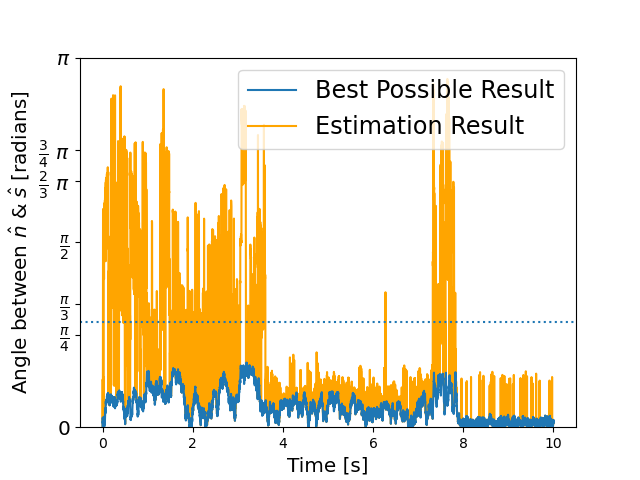
\includegraphics[width=\textwidth]{./Images/fig7b.png}
	\end{subfigure}
	\caption{Simulation results of: (a) the dimer's orientation vector with time, (b) the dimer's [x,y,z] position with time.}
	\label{fig:motion}
\end{figure}

In the simulations of Vigilante~\emph{et~al}.\ \cite{Vigilante2020Brownian_OT}, trapped symmetrical dimers were investigated; their findings showed that the optical torque on the dimer goes to zero while aligned vertically and is at its maximum in a horizontal alignment. However as seen in Figure~\ref{fig:motion} asymmetric dimers demonstrate dynamics that do not immediately achieve steady state. We chose to use asymmetric dimers as our benchmark due to this fact, as its orientational motion is far more complex than a symmetric dimer. In the future we hope to further investigate the motion of asymmetric dimers. 
%%%%%%%%%%%%%%%%%%%%%%%%%%%%%%%%%%%%%%%%%%%%%%%%%%%%%%%%%%%%%%%%%%%%%
%%%%%%%%%%%%%%%%%%%%%%%%%%%%%%%%%%%%%%%%%%%%%%%%%%%%%%%%%%%%%%%%%%%%%
\subsection{Accounting for sources of error in light scattering measurements}
When it comes to analysing light scattering from any size particle, error analysis becomes a significant factor. Typically this can be accounted for by averaging over long periods of time to get an assessment of the steady state conditions of the target particle. However in our case where we wish to know the instantaneous orientation, we instead have to rely on our understanding of how uncertainty can effect our model's performance. We identified two areas which are likely sources of error in our estimation: firstly, an incorrect modelling of the target particle, and secondly, signal noise arising from experimental factors. We highlight how we address these areas below. 
%%%%%%%%%%%%%%%%%%%%%%%%%%%%%%%%%%%%%%%%%%%%%%%%%%%%%%%%%%%%%%%%%%%%%
\subparagraph{Impact of incorrect dimer sizing}
\label{sec:lam}

One of the main limitations of our model is that we assume that the dimer being modelled in MSTM is accurate to the dimer being trapped in the optical tweezer. Sizing molecules accurately is a significant challenge for single particle analysis so there is bound to be some uncertainty with the measurements. We ran our model 3 times with the neural net being trained on a dimer of size ratio $1:1.95$, $1:2.00$ and $1:2.05$.

\begin{figure}[h]
	\centering
	\begin{subfigure}{0.33\textwidth}
			\subcaption{}
			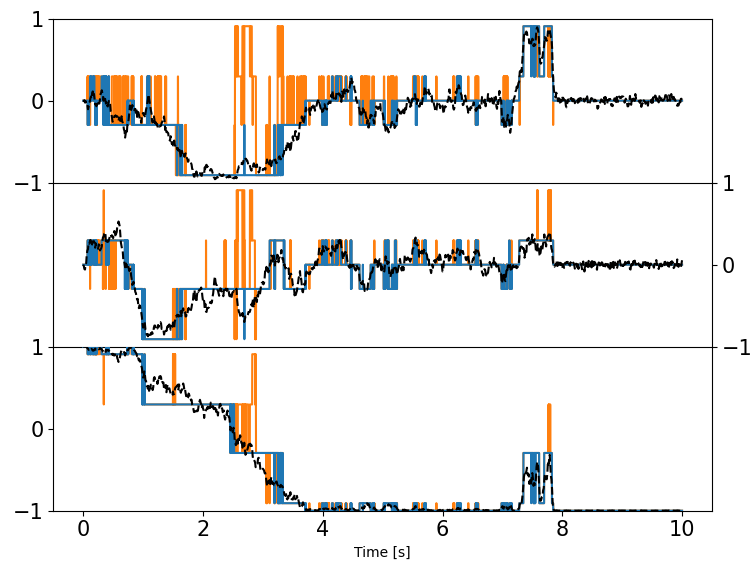
\includegraphics[width =\textwidth]{./Images/fig8a.png}
	\end{subfigure}
	\begin{subfigure}{0.31\textwidth}
		\subcaption{}
		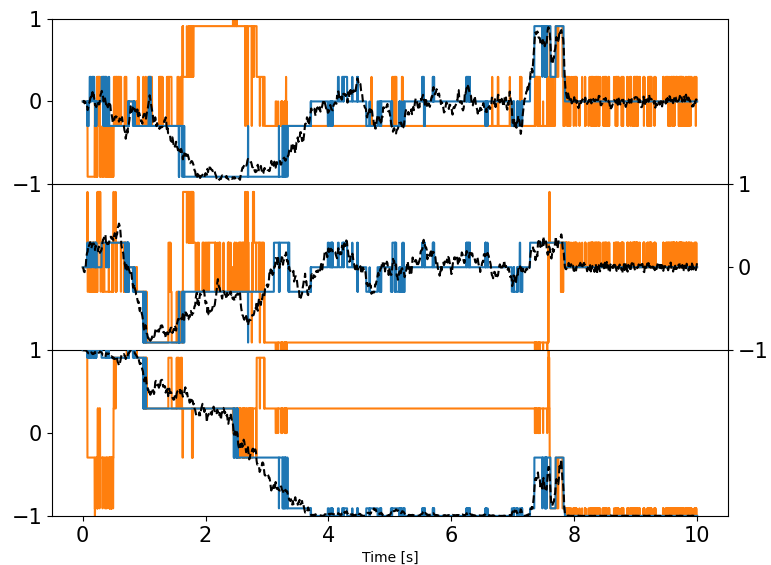
\includegraphics[width=\textwidth]{./Images/fig8b.png}
	\end{subfigure}
	\begin{subfigure}{0.31\textwidth}
		\subcaption{}
		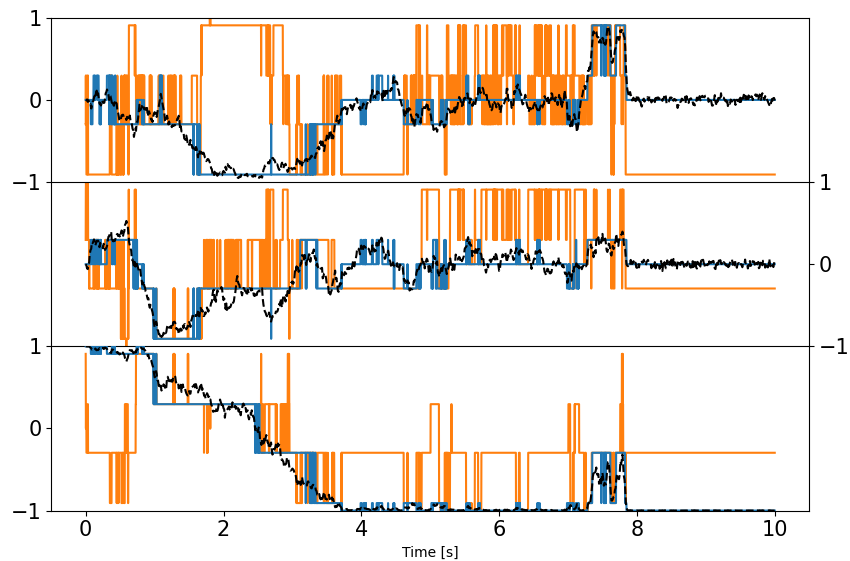
\includegraphics[width=\textwidth]{./Images/fig8c.png}
	\end{subfigure}
	\caption{Model estimates of orientation when neural net has been trained on dimer of size ratio: (a) 1:2 $[F(K_l)=9.456]$, (b) 1:2.05 $[F(K_l)=1.324]$, (c) 1:1.95 $[F(K_l)=1.325]$ ($n_{refs} = 30$)}
	\label{fig:size}
\end{figure}
As can be seen from Fig~\ref{fig:size}  even the slightest change in size ratio makes a very significant difference to the performance of our model. This amounts to just over $100 nm$ in the dimer's overall size, yet results in our model being correct from over 90 \% of the time to now as low as 30 \%. This highlights the importance of correctly sizing trapped entities before performing any in depth analysis of the scattering pattern, as even the slightest deviation can have a serious impact. We addressed this by increasing the number of available reference points from 30 to 126 (following the same procedure as given by \cite{Rey2006} to evenly space out the coordinates) and increasing the weighting factor in Eq~\ref{eq:boltz}. While this didn't have a significant improvement on the overall accuracy of the model, in the worst case having a slight increase from 30.5 \% to 40.3 \%, it did help to significantly reduce the magnitude between our model's estimations and the dimer's motion as seen below in Fig~\ref{fig:refs}.
\begin{figure}[h]
	\centering
	\begin{subfigure}{0.31\textwidth}
		\subcaption{}
		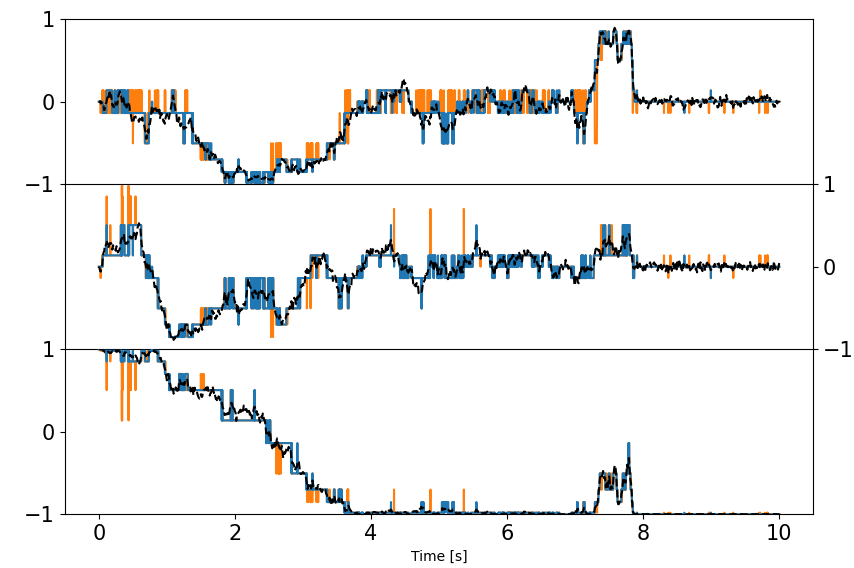
\includegraphics[width =\textwidth]{./Images/fig9a.png}
	\end{subfigure}
	\begin{subfigure}{0.31\textwidth}
		\subcaption{}
		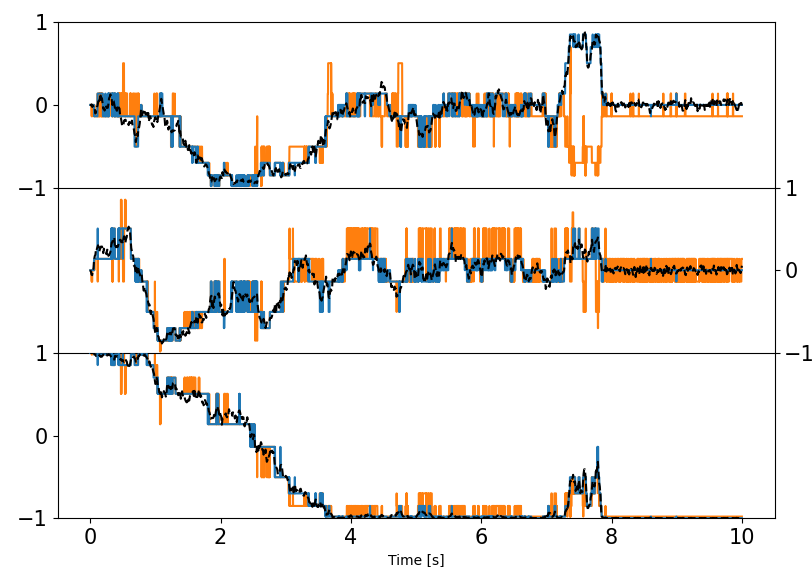
\includegraphics[width=\textwidth]{./Images/fig9b.png}
	\end{subfigure}
	\begin{subfigure}{0.31\textwidth}
		\subcaption{}
		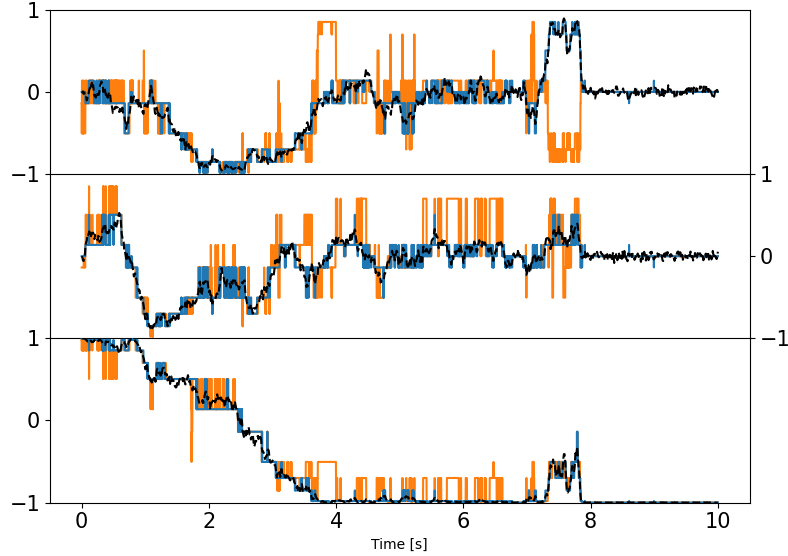
\includegraphics[width=\textwidth]{./Images/fig9c.png}
	\end{subfigure}
	\caption{Model estimates of orientation when neural net has been trained on dimer of size ratio: (a) 1:2 $[F(K_l)=11.756]$, (b) 1:2.05 $[F(K_l)=1.233]$, (c) 1:1.95 $[F(K_l)=2.128]$, ($n_{refs} = 126$)}
	\label{fig:refs}
\end{figure}

Notably the increasing the number of reference orientations had a greater effect when our neural network was trained on a 1:1.95 dimer than a 1:2.05 dimer. This suggests that overshooting our size estimate will be less detrimental to our estimation. Notably if the our sizing is off the neural network does not predict a smooth motion within the trap; instead predicting that the dimer is jumping back and forth between different orientations. This suggest that we can narrow down our estimate of the particle's size by assessing how the dimer is reorienting within the trap, as we should expect a smooth continuos prediction. Since we are working with a spherical dimer it also stands to reason that techniques such as image analysis could be used in part to address this, so long as the trapped entity is sufficiently illuminated. 
%%%%%%%%%%%%%%%%%%%%%%%%%%%%%%%%%%%%%%%%%%%%%%%%%%%%%%%%%%%%%%%%%%%%%
\subparagraph{Impact of measurement noise on model predictions}
\label{sec:epsilon}

So far a key assumption of the neural network implementation is that the detected scattering signal has no uncertainty associated with it. In reality of course scattering signals will always have some non-zero measurement noise. This can be attributed to a variety of factors, from a measurement bias in the detector, to the Brownian motion of the dimer itself. To explore the impact of measurement uncertainty on orientation estimation model performance we introduce a Gaussian noise to the measured signal:
\begin{align}
	I(\hat{\bf s}) = I(\hat{\bf s}) \pm \epsilon I(\hat{\bf s})
\end{align}
where $\epsilon$ is the percentage error associated with the scattering signal. Figure~\ref{fig:epsilon} shows the performance of the model at a range of $\epsilon$ using in-plane detector angles $15^{\circ}$, $55^{\circ}$, $90^{\circ}$ and out-of-plane detector at $75^{\circ}$, with $\beta$ set to $1$:

\begin{figure}[h]
	\centering
	\begin{subfigure}{0.32\textwidth}
		\subcaption{}
		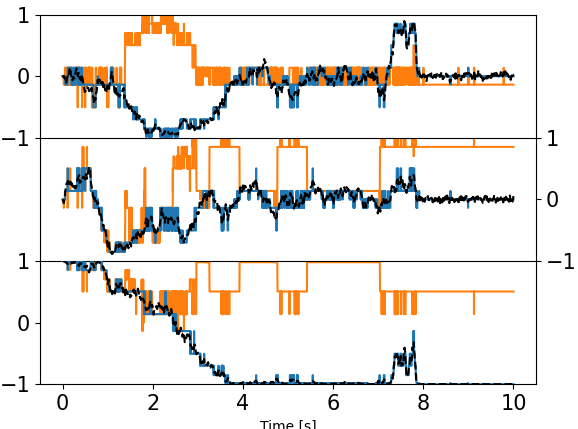
\includegraphics[width=\textwidth]{./Images/fig10a.png}
	\end{subfigure}
	\begin{subfigure}{0.32\textwidth}
		\subcaption{}
		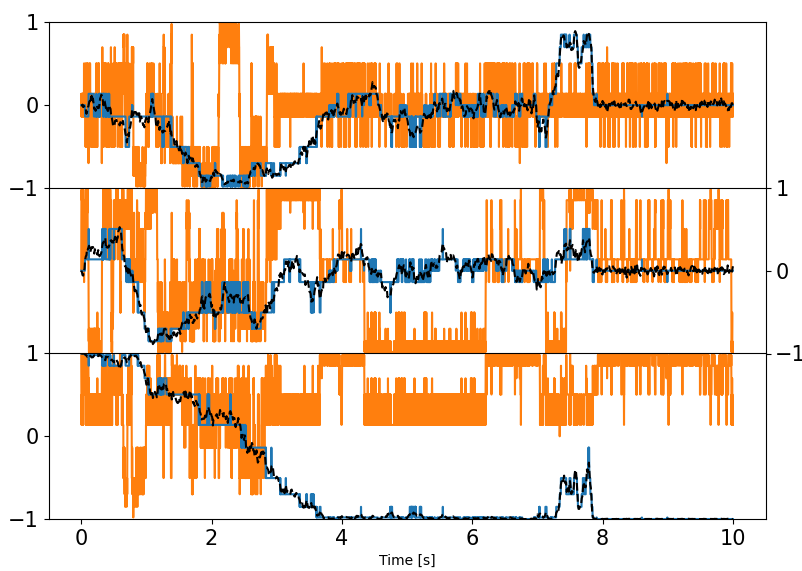
\includegraphics[width=\textwidth]{./Images/fig10b.png}
	\end{subfigure}
	\begin{subfigure}{0.32\textwidth}
		\subcaption{}
		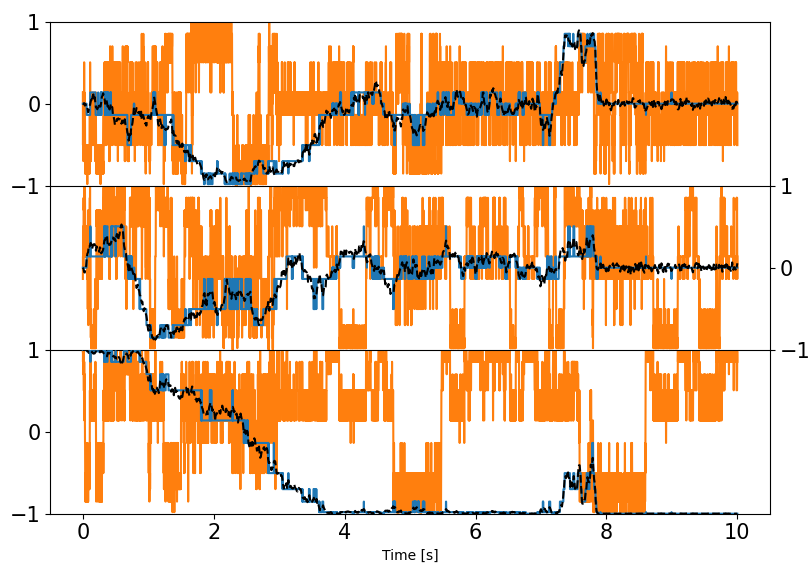
\includegraphics[width=\textwidth]{./Images/fig10c.png}
	\end{subfigure}
	\caption{Model prediction for signal error of (a) $1\%$ ~  $[F(K_l)=7.246]$, (b) $15\%$ $[F(K_l)=0.511]$, and (c) $25\%$ ~  $[F(K_l)=0.536]$.}
	\label{fig:epsilon}
\end{figure}

As can be seen from Figure~\ref{fig:epsilon}, the inclusion of signal noise quickly leads to a decrease in the model's performance. This is due to an inherent feature of the inverse scattering problem: two distinct regions in orientation space can become heavily intertwined and thus no longer well separated when mapped to intensity space (even though the mapping remains continuous): so even small uncertainties in the scattering data can lead to large 'mistakes' in the choice of orientation by the neural network. (Indeed if this was not the case the inverse scattering problem would be quite simple.) 

To reduce the effects of the signal noise we took the time average of the expected signal over 0.02s and then had our neural network estimate the orientation based on the average signal.
\begin{figure}[h]
	\centering
	\begin{subfigure}{0.32\textwidth}
		\subcaption{}
		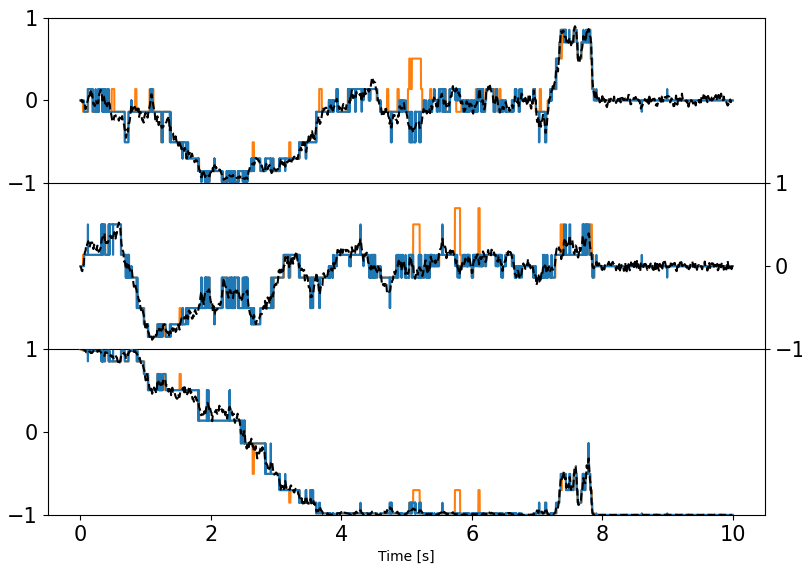
\includegraphics[width=\textwidth]{./Images/fig11a.png}
	\end{subfigure}
	\begin{subfigure}{0.32\textwidth}
		\subcaption{}
		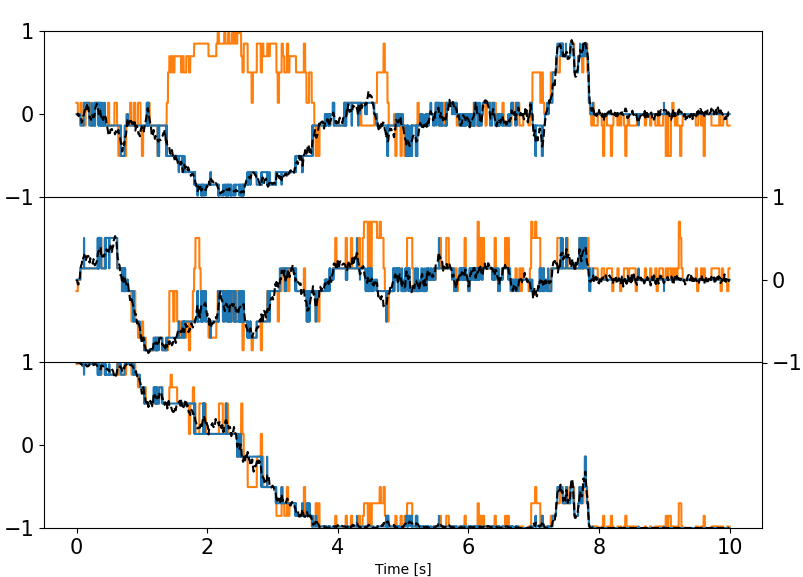
\includegraphics[width=\textwidth]{./Images/fig11b.png}
	\end{subfigure}
	\begin{subfigure}{0.32\textwidth}
		\subcaption{}
		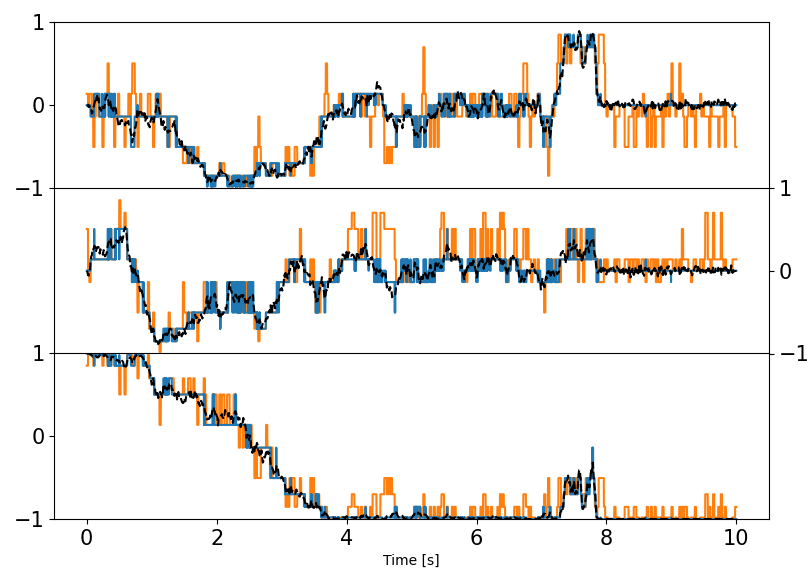
\includegraphics[width=\textwidth]{./Images/fig11c.png}
	\end{subfigure}
	\caption{Model prediction for signal error of (a) $1\%$ $[F(K_l)=4.823]$,  (b) $15\%$ $[F(K_l)=1.494]$, and (c) $25\%$ $[F(K_l)=0.882]$, time averaged over $20\,{\rm ms}$}
	\label{fig:time average}
\end{figure}
This resulted in a reduction in the overall signal noise and provided a higher degree of accuracy for our model. There appears to be no clear correlation between the length over which we time average and the performance of our model. Time averaging over every 0.05s resulted in a drastically worse performance; this is due to the fact that over longer time periods there is greater uncertainty regarding how the dimer's orientation has changed, thus tracking the instantaneous orientation becomes harder for the neural network. Fortunately, time averaging even over $20\,{\rm ms}$ seems to provide a satisfactory estimation of the dimer's angular dynamics within the optical trap. 

%%%%%%%%%%%%%%%%%%%%%%%%%%%%%%%%%%%%%%%%%%%%%%%%%%%%%%%%%%%%%%%%%%%%%
%%%%%%%%%%%%%%%%%%%%%%%%%%%%%%%%%%%%%%%%%%%%%%%%%%%%%%%%%%%%%%%%%%%%%
\section{Conclusion}
\label{sec:Conclusion}

We have developed a method for measuring the dynamics of an optically-trapped 'complex object' based purely on limited measurements of the object's light scattering at a small number of detection angles. We demonstrate the method using the orientation of an asymmetric dimer as the dynamical variable and object of interest, but in principle the model can be applied to any characteristic that impacts the light scattering pattern produced by a trapped entity. The MSTM package is a flexible tool for calculating the light scattering of complex objects using a representation of the object as a set of micro-particles, enabling training of a neural network to enable categorisation of the mapping between scattering and trapped object characteristics. By taking account of knowledge about the physically realistic behaviour of the trapped object and the characteristics of the trap (which impact the dynamics of the object), the Bayesian inference method can be refined to provide a reliable estimation of object characteristics of interest, even in the presence of measurement noise. Fundamentally the inverse scattering problem is difficult to solve since the mapping between object characteristics and scattering can be highly complex: but Bayesian inference based on neural network estimation of the mapping provides a powerful method for practical applications, extending the use of optical trapping beyond measuring microscopic force response toward detailed structural and dynamic information about complex trapped entities.\\

Here we simplify the problem somewhat by employing a relatively small finite number of 'reference orientations' to map between scattering and dimer orientation: the precision of estimation could be improved by utilising a greater number of reference orientations, although there remains a balance between the realisable precision of orientation estimate and the noise level of the scattering measurement. Another avenue to further explore would be using the method to optimise the choice of detection angles, essentially to find the region in the mapping between measured scattering and orientation that offers the best degree of confidence through optimal separation of scattering signals for distinct orientations. For \textit{sequences} of data such as dynamic measurements, a further potential enhancement would be to consider more complex correlations based on prior expectations of the dynamics. Here already we improve the method using a non-uniform prior based on only the immediately previous measurement in time (see Section \ref{sec:Bayes}): considering more detailed correlations such as multiple previous timesteps is likely to further enhance the reliability of the estimation.


%%%%%%%%%%%%%%%%%%%%%%%%%%%%%%%%%%%%%%%%%%%%%%%%%%%%%%%%%%%%%%%%%%%%%%%%%%%%%%%%
%%%%%%%%%%%%%%%%%%%%%%%%%%%%%%%%%%%%%%%%%%%%%%%%%%%%%%%%%%%%%%%%%%%%%%%%%%%%%%%%
\noindent \textbf{Acknowledgement.} The authors thank the support for this research from the funding provided by the Leverhulme Trust. \\
  
\noindent \textbf{Disclosures.} The authors declare no conflict of interest. \\


%%%%%%%%%%%%%%%%%%%%%%%%%%%%%%%%%%%%%%%%%%%%%%%%%%%%%%%%%%%%%%%%%%%%%%%%%%%%%%%%
%%%%%%%%%%%%%%%%%%%%%%%%%%%%%%%%%%%%%%%%%%%%%%%%%%%%%%%%%%%%%%%%%%%%%%%%%%%%%%%%
\bibliography{bib} 
\bibliographystyle{ieeetr}

\newpage
\appendix
\onecolumn
%%%%%%%%%%%%%%%%%%%%%%%%%%%%%%%%%%%%%%%%%%%%%%%%%%%%%%%%%%%%%%%%%%%%%
%%%%%%%%%%%%%%%%%%%%%%%%%%%%%%%%%%%%%%%%%%%%%%%%%%%%%%%%%%%%%%%%%%%%%
\section*{Appendix}
\setcounter{table}{0}
\renewcommand{\thetable}{A\arabic{table}}
\begin{table}[h]
	\begin{center}
		\caption{\label{tab:A1}
		%
		Reference Orientations vector components, for $n_{refs} = 30 \ ^*$}
		\begin{tabularx}{0.65\textwidth}{
				| >{\centering\arraybackslash}X
				| >{\centering\arraybackslash}X
				| >{\centering\arraybackslash}X
				| >{\centering\arraybackslash}X | }
			\hline\hline
			$\alpha$ & $\hat{\bf n}_{\alpha,\ x}$ &  $\hat{\bf n}_{\alpha,\ y}$ &  $\hat{\bf n}_{\alpha,\ z}$ 
			\\ \hline
			\csvreader[
			head to column names
			]
			{./data/n_list.csv}{}{
			\index\ & \nx\ & \ny\ & \nz\ \\
			} \\
			\hline\hline 
		\multicolumn{4}{l}{\small *Orientation vector points from centre of sphere 1 to centre of sphere 2.} \\
		\end{tabularx}
\end{center}
\end{table}
%%%%%%%%%%%%%%%%%%%%%%%%%%%%%%%%%%%%%%%%%%%%%%%%%%%%%%%%%%%%%%%%%%%%%
\newpage
\begin{table}[h]
	\begin{center}
		\caption{\label{tab:A2}
			% 
			Raw intensities $I_k^*$ and scaled intensities $y_k$}
		\begin{tabular}{|c|c|c|c|c|c|c|}
			\hline\hline
			$\alpha$  & $I(\hat{\bf n}_\alpha\ ,\ 15^{\circ})$ &  $I(\hat{\bf n}_\alpha \ , \ 55^{\circ})$ &  $I(\hat{\bf n}_\alpha \ ,\ 90^{\circ})$ & $y(\hat{\bf n}_\alpha \ , \ 15^{\circ})$ & $y(\hat{\bf n}_\alpha \ , \ 55^{\circ})$ & $y(\hat{\bf n}_\alpha \ , \ 90^{\circ})$ \\
		    \hline
			\csvreader[
			head to column names
			]
			{./data/y_list.csv}{}{
				\index\ & \Ix\ & \Iy\ & \Iz\ & \yx\ & \yy\ & \yz\ \\
			} \\
			\hline\hline 
			\multicolumn{7}{l}{\small *$I_k$ values are calculated using MSTM package.} \\
		\end{tabular}
	\end{center}
\end{table}

%%%%%%%%%%%%%%%%%%%%%%%%%%%%%%%%%%%%%%%%%%%%%%%%%%%%%%%%%%%%%%%%%%%%%
%%%%%%%%%%%%%%%%%%%%%%%%%%%%%%%%%%%%%%%%%%%%%%%%%%%%%%%%%%%%%%%%%%%%%
%%%%%%%%%%%%%%%%%%%%%%%%%%%%%%%%%%%%%%%%%%%%%%%%%%%%%%%%%%%%%%%%%%%%%
\end{document}
\endinput
